\subsection{开发环境}
开发环境包括编程语言、软件环境、硬件环境等。
\begin{table}[H]
\begin{adjustwidth}{-3cm}{-3cm}
\begin{center}
\begin{tabular}{|p{.2\textwidth}| p{.8\textwidth}|} \hline
计算逻辑 & Python2.7  \\ \hline
前端框架 & Flask  \\ \hline
前端展示 & HTML5  \\ \hline
数据库 & MySQL \\ \hline

系统 & Ubuntu 16.04.3 LTS  \\ \hline

处理器 & Ubuntu Intel Core5  \\ \hline
\end{tabular}
\end{center}
\end{adjustwidth}
\end{table}



\subsection{数据来源}
\begin{itemize}
\item 国泰安CSMAR数据库专注于学术高校研究

\item 覆盖经济、股票、基金、债券等领域,涵盖面广。

\item 数据做深层衍生加工,而CSMAR侧重于数据的深度,强调对原始数据的深层专业加工、整理,属精准数据。

\item CSMAR支持EXCEL、TXT、XML、 SAS 、STATA 、MATLAB 、R等多种格式。

\end{itemize}

\subsection{数据结构}
本系统使用了352万条数据,以进行大数据情况下的系统性能测试。
\begin{table}[H]
\begin{adjustwidth}{-3cm}{-3cm}
\begin{center}
\begin{tabular}{|p{.3\textwidth}| p{.7\textwidth}|} \hline
债券基本情况表 & 据总记录数:104949,记录区间:1990-2017  \\ \hline
债券日交易信息表 & 数据总记录数:3524198,数据开始时间:1996-2017
存储债券每日交易信息,包括价格,成交量,涨跌幅等
 \\ \hline
\end{tabular}
\end{center}
\end{adjustwidth}
\end{table}

Figure \ref{fig:sys.param}为数据结构示意图。
\begin{figure}[H]
\begin{center}
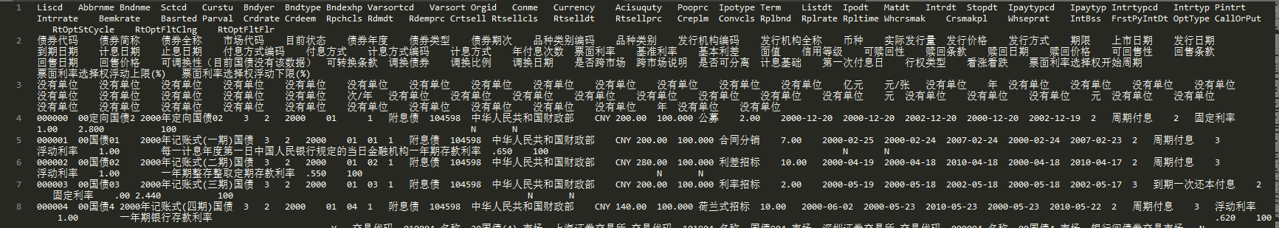
\includegraphics[width=16cm]{img//DataStructure.PNG}
\caption{数据结构示意图}
\label{fig:sys.param}
\end{center}
\end{figure}



\subsection{数据库设计}
本系统使用MySQL数据库。
\begin{table}[H]
\begin{adjustwidth}{-3cm}{-3cm}
\begin{center}
\begin{tabular}{|p{.3\textwidth}| p{.7\textwidth}|} \hline
债券基本情况表 & 主键:债券id  \\ \hline
债券日交易信息表 & 主键:债券id+交易日期\\ \hline
\end{tabular}
\end{center}
\end{adjustwidth}
\end{table}


\subsection{数据库性能}
我们测试了数据库在不同情况下的处理速度。
\begin{table}[H]
\begin{adjustwidth}{-3cm}{-3cm}
\begin{center}
\begin{tabular}{|p{.3\textwidth}| p{.7\textwidth}|} \hline
实验目的 & 测试数据库对大量请求响应的处理速度  \\ \hline
实验过程 &给出10000个(债券id,交易时间),由数据库取出最相似的交易信息\\ \hline
\end{tabular}
\end{center}
\end{adjustwidth}
\end{table}

Figure \ref{fig:sys.param}为使用全Varchar字段情况。
\begin{figure}[H]
\begin{center}
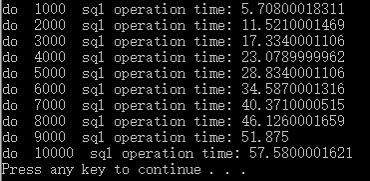
\includegraphics[width=16cm]{img//Varchar.PNG}
\caption{使用全Varchar字段情况}
\label{fig:sys.param}
\end{center}
\end{figure}

Figure \ref{fig:sys.param}为使用int类型和data类型情况。
\begin{figure}[H]
\begin{center}
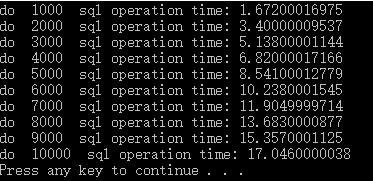
\includegraphics[width=16cm]{img//int_data.PNG}
\caption{使用int类型和data类型情况}
\label{fig:sys.param}
\end{center}
\end{figure}

Figure \ref{fig:sys.param}为多个query组合情况。
\begin{figure}[H]
\begin{center}
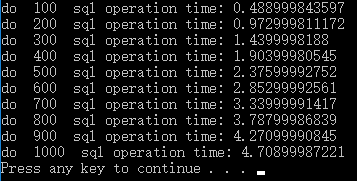
\includegraphics[width=16cm]{img//multi_query.PNG}
\caption{多个query组合情况}
\label{fig:sys.param}
\end{center}
\end{figure}

Figure \ref{fig:sys.param}为不同情况下数据库性能比较。
\begin{figure}[H]
\begin{center}
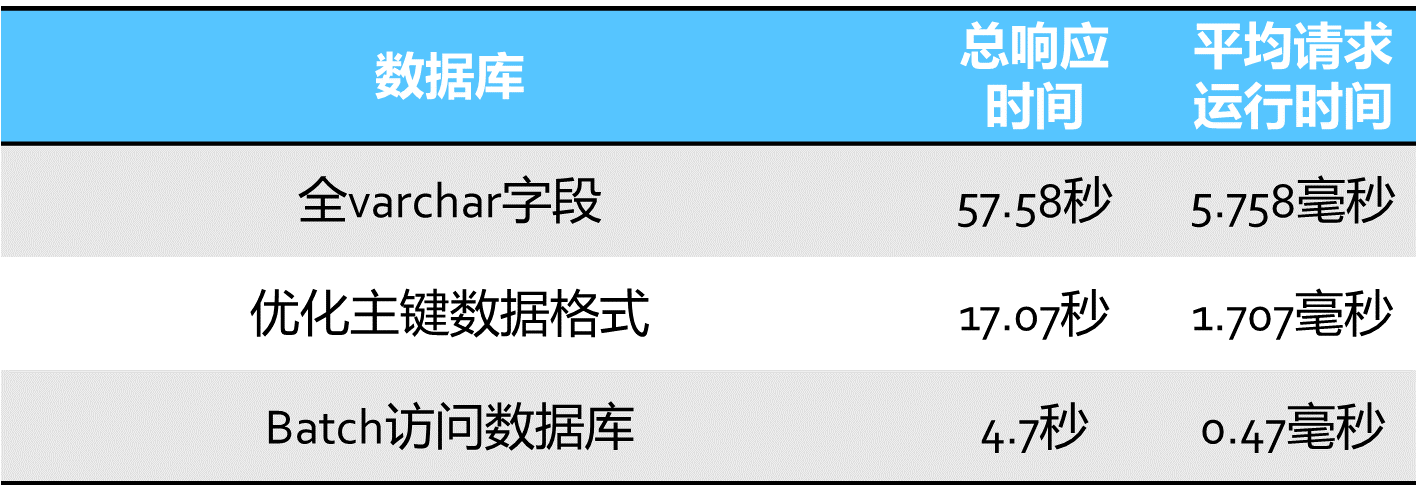
\includegraphics[width=16cm]{img//DB_performance.PNG}
\caption{不同情况下数据库性能比较}
\label{fig:sys.param}
\end{center}
\end{figure}

\subsection{数据测试集}
为了对该系统的性能进行测试,我们模拟生成了100万条债券数据。数据格式为json格式,包括6项数据:
\begin{enumerate}
\item 发行时间
\item 年限
\item 付息频率
\item 面值
\item 付息利率
\item 出售时间
\end{enumerate}

Figure \ref{fig:sys.param}为数据的Json格式。
\begin{figure}[H]
\begin{center}
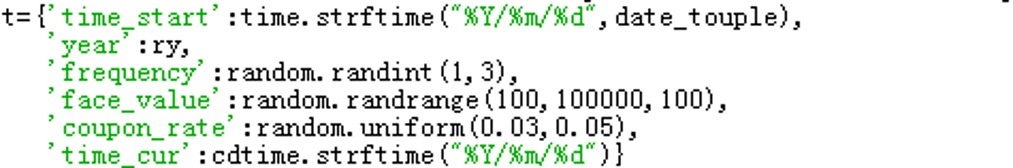
\includegraphics[width=16cm]{img//test_data.PNG}
\caption{数据的Json格式}
\label{fig:sys.param}
\end{center}
\end{figure}